\documentclass{article}

% Language setting
% Replace `english' with e.g. `spanish' to change the document language
\usepackage[english]{babel}


% Set page size and margins
% Replace `letterpaper' with `a4paper' for UK/EU standard size
\usepackage[a4paper, top=2cm,bottom=2cm,left=3cm,right=3cm,marginparwidth=1.75cm]{geometry}

% Useful packages
\usepackage{amsmath,amsfonts}
\usepackage{graphicx,caption}
\usepackage{authblk}
\usepackage{float}
\usepackage[colorlinks=true, allcolors=blue]{hyperref}
\usepackage{natbib}
\usepackage{indentfirst}
\usepackage{amsmath}
% \usepackage{palatino}

\title{A Mathematical Model for Human Fecundability and Aneuploidy-driven Pregnancy Loss}

\author[1]{Arjun Biddanda}
\author[1]{Sara A. Carioscia}
\author[1]{Rajiv C. McCoy}
\affil[1]{Department of Biology, Johns Hopkins University}

\begin{document}
\maketitle

\section*{Model Description}

In the original model from \citep{Macklon2002-zn}, the ``iceberg'' of pregnancy loss probabilities is framed as the \textit{absolute} probability of the pregnancy loss outcome (\ref{fig:1}). However, in many ways it may be more favorable to model the series of \textit{conditional} probabilities that underlie each section of the iceberg. 

\begin{figure}[H]
\begin{center}
    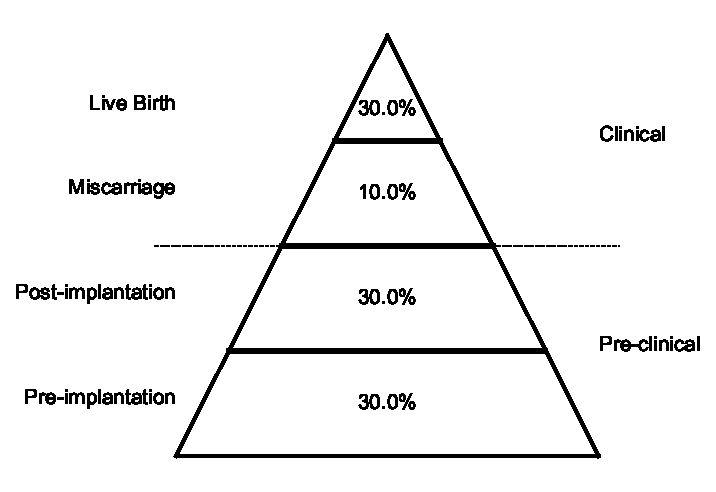
\includegraphics[width=0.5\textwidth]{figures/macklon_recreate.041724.pdf}
\end{center}
\vspace{-1.5em}
\caption{The ``Iceberg'' of pregnancy loss (repurposed from \citep{Macklon2002-zn}).}
\label{fig:1}
\end{figure}

We provide an introduction to the model below, with the conditional probabilities. The  probability we would like to model is the probability of a \textit{live birth conditional on conception occurring}. We model this using a series of conditional probabilities: 

\begin{equation}
	P(\text{Live Birth}) =  (1 - P(\text{Miscarriage} | \text{no EPL})) \cdot (1 - P(\text{EPL} | \text{implantation})) \cdot (1 - P(\text{failed implantation}))
\end{equation}

This model posits that a health live birth (conditional on conception occurring) is conditional on no implantation failure, no early pregnancy loss, \textit{and} no miscarriages.

While there may be a number of potential factors influencing both of these negative events during pregnancy, we primarily focus on the assumption that aneuploidy drives a large fraction of these effects. We first posit that the distribution of aneuploidy outcomes come from the following distribution $P(A,M)$: 

% \begin{equation}
% \begin{aligned}
% P(\text{A}_{Meiotic} = a, \text{A}_{Mitotic} = m) &= \begin{cases}
% 206 / 909 = 0.226 &, a = \text{Euploid}, m = \text{None}\\
% (88 + 61)/ 909 \times 3/4 = 0.123 &, a = \text{Euploid}, m = \text{Early-Mitotic}\\
% (88 + 61)/ 909 \times 1/4 = 0.041 &, a = \text{Euploid}, m = \text{Late-Mitotic}\\
% 294 / 909 = 0.32 &, a = \text{Meiotic}, m = \text{None}\\
% 260 / 909 \times 3/4 = 0.215 &, a = \text{Meiotic}, m = \text{Early-Mitotic}\\
% 260 / 909 \times 1/4 = 0.072 &, a = \text{Meiotic}, m = \text{Late-Mitotic}
% \end{cases}
% \end{aligned}
% \end{equation}

\begin{table}[H]
\begin{center}
	\begin{tabular}{ |c|c|c| } 
	 \hline
	  & Meiotic & Euploid  \\ 
	 \hline
	 None & $\frac{294}{909}$ & $\frac{206}{909}$ \\ 
	 \hline
	 Early-Mitotic & $\frac{260}{909}\times \frac{3}{4}$ & $\frac{(88 + 61)}{909}\times \frac{3}{4}$ \\
	 \hline
	 Late-Mitotic & $\frac{260}{909}\times \frac{1}{4}$ & $\frac{(88 + 61)}{909}\times \frac{1}{4}$\\
	 \hline
	\end{tabular}
	\caption{Joint probability distribution of meiotic (columns) and mitotic (rows) aneuploidy based on outcome data from \citep{McCoy2023-dg}.}
	\label{table:1}
	\end{center}
\end{table}

We have chosen specifically to model the joint distribution of \textit{both} mitotic and meiotic aneuploidies since they both contribute to early pregnancy loss (particular meiotic aneuploidies and early-mitotic aneuploidies). We note that we have also roughly approximated a ratio of 3:1 of early to late-mitotic errors as the first cell divisions post-fertilization are those that are most prone to errors. As long as all elements of the joint probability distribution satisfy being a full probability distribution, then this can be pre-supposed (see later section on scaling for maternal age). 

\subsubsection*{Implantation Failure}

The second conditional model is the implantation failure rate: 

\begin{equation}
P(\text{failed implantation} | A=a, M=m) = \begin{cases}
0.16 &, a = \text{Euploid}, m = \text{None}\\
0.36 &, a = \text{Meiotic}, m = \text{None}\\
0.57 &, a = \text{Euploid}, m = \text{Early-Mitotic}\\
0.55 &, a = \text{Meiotic}, m = \text{Early-Mitotic}\\
0.16 &, a = \text{Euploid}, m = \text{Late-Mitotic}\\
0.36 &, a = \text{Meiotic}, m = \text{Late-Mitotic}\\
\end{cases}
\end{equation}

This conditional probability suggests that different forms of aneuploidy have different impacts on implantation - roughly corresponding to when they arise during development (e.g. meiotic-origin being the earliest).  We have approximated the rate of implantation failure here as the probability of embryo arrest from \citep{McCoy2023-dg} (Figure 4B) -- however there may be other reasons beyond aneuploidy for implantation to fail. We also note that in this model the conribution of later-occurring \textit{mitotic} aneuploidies are effectively limited.   

We can then calculate the following absolute probability:

\begin{equation}
P(\text{failed implantation}) = \gamma_{implant} + \sum_{A}\sum_{M} P(\text{failed implantation} | A, M) P(A, M) ,
\end{equation}

which directly corresponds to the bottom section of the iceberg in \citep{Macklon2002-zn}, but importantly now incorporates different types of aneuploidy. We have also added an intercept term ($\gamma_{implant}$) that acts as a kind of catch-all term for the pregnancy loss that can occur at this stage.   

\subsubsection*{Early Pregnancy Loss}

We now turn to the second conditional probability for early pregnancy loss (EPL) which is when there is pregnancy loss following a successful implantation but prior to being a clinically-defined miscarriage.

\begin{equation}
	P(EPL | \text{implantation}, A=a, M=m) = \begin{cases}
	\epsilon &, a= \text{Euploid}, m=\text{None}\\
	0.57 &, a = \text{Meiotic}, m=\text{None}\\
	1 - \eta &, a = \text{Euploid}, m=\text{Early-Mitotic}\\
	1 - \eta &, a = \text{Meiotic}, m=\text{Early-Mitotic}\\
	\epsilon &, a = \text{Euploid}, m=\text{Late-Mitotic}\\
	0.57 &, a = \text{Meiotic}, m=\text{Late-Mitotic}\\
	\end{cases},
\end{equation}

where $\eta$ is an "escape" probability where a meiotic or mitotic aneuploidy does not lead to early-pregnancy loss and $\epsilon$ is the probability of lethal mutations that may lead to early pregnancy loss outcomes even within a euploid embryo (or euploid + late mitotic embryo). The probability of 0.57 comes from \citep{Gu2021-tk}\footnote{The parameter $\epsilon$ represents the probability of smaller scale, but still lethal, structural variants so can be thought of as a larger catch-all for lethal mutations that survive implantation but still lead to inviability}. 

The corresponding absolute probability for this section of the ``iceberg'' is: 

\begin{equation}
\begin{aligned}
P(EPL) &=  \gamma_{EPL} + \sum_{A}\sum_{M} P(EPL | \text{implantation}, A, M) \\
&\cdot (1 - P(\text{failed implantation} | A, M) - \gamma_{implant})\\ 
&\cdot P(A, M),
\end{aligned}
\end{equation}

where we have again added in a baseline level of early pregnancy loss that is not conditional on aneuploidy ($\gamma_{EPL}$). 

\subsubsection*{Miscarriage}

The final consideration is the conditional probability of a miscarriage, conditional on surviving beyond EPL and implantation. 

\begin{equation}
	P(Miscarriage | \text{Aneuploidy}=a) = \begin{cases}
	0.3 &, a= \text{Euploid}\\
	0.3 &, a = \text{Meiotic}\\
	0.3 &, a = \text{Mitotic}\\
	\end{cases},
\end{equation}

In most cases however, we do not have strong estimates for whether the miscarriage was the result of an aneuploidy or not. However, in almost all birth cohort datasets the occurrence of miscarriages reflects a strong U-shaped trend  with maternal age \citep{Gruhn2019-al}. 

We then perform a similar marginalization as before - to get the full probability of miscarriage: 

\begin{equation}
\begin{aligned}
P(\text{Miscarriage}) &=  \gamma_{Miscarriage} + \sum_{A}\sum_{M} P(Miscarriage | A,M)\\
&\cdot (1. - P(EPL | \text{implantation}, A, M) - \gamma_{EPL})\\
&\cdot (1 - P(\text{failed implantation} | A, M) - \gamma_{implant})\\ 
&\cdot P(A, M),
\end{aligned}
\end{equation}


\subsubsection*{Accounting for Maternal Age} 

Since maternal age has a well-documented effect on the abundance of \textit{meiotic} aneuploidies, here we focus on how to scale the original $P(A,M)$ distribution such that the distribution of $P(A = \text{Meiotic})$ can scale as a function of maternal age - whereas the rate of mitotic errors will remain constant as a function of age. Corroborating the total proportion of meiotic aneuploid embryos with the fitted probability of meiotic trisomy in \citep{Gruhn2019-al}, we get approximate maternal age of 46.20 to 47.75 years - significantly higher than the realized 38.9 year average maternal age. 

Under the assumption that the mean maternal age of the patients in \citep{McCoy2023-dg} is $\sim 38.9$ years of age, we scale the marginal probability of a meiotic error $P(A) = \sum_M P(A,M)$ by $\alpha_{age} = \frac{P(M | age)}{P(M | age = 38.9)}$ using the fitted model from \citep{Gruhn2019-al}.

\section*{Results}

Following these model approximations - we can estimate how aneuploidy occurrence shapes the distribution of pregnancy losses at various stages in development. The resulting output of this model is a way to generate maternal age specific ``icebergs'' for pregnancy loss risk and fecundability, or the tip of the iceberg (\ref{fig:2}). 

\begin{figure}[H]
\begin{center}
    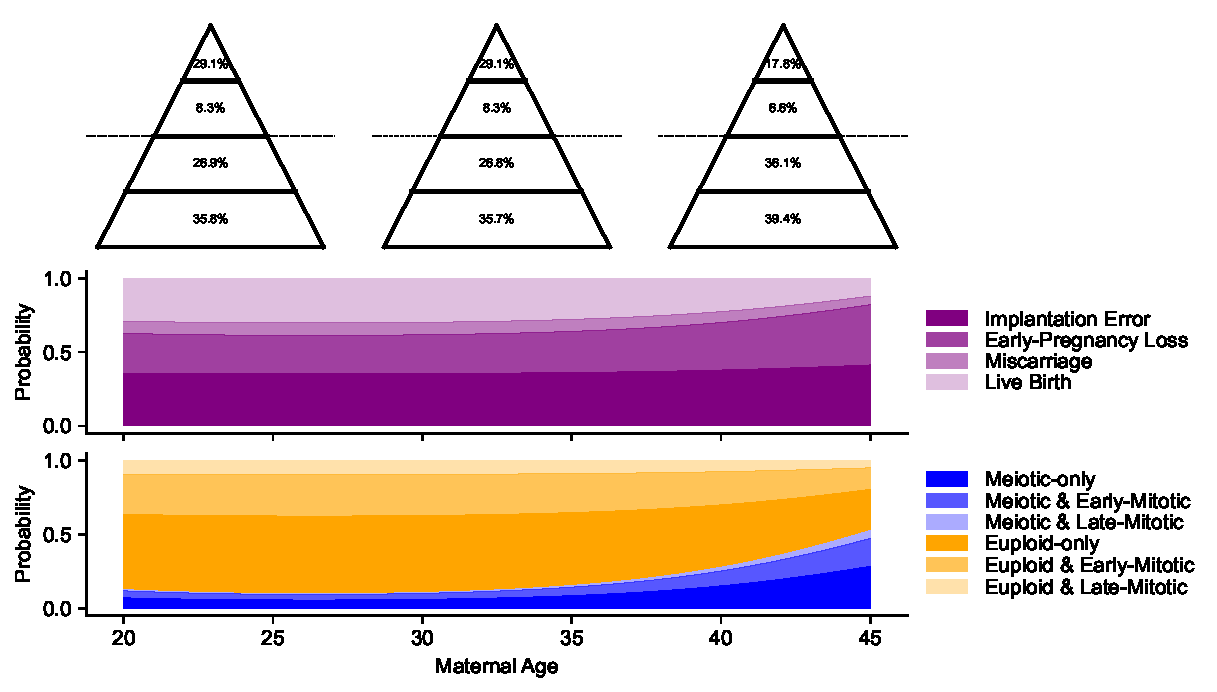
\includegraphics[width=0.75\textwidth]{figures/model_figure.042024.pdf}
\end{center}
\vspace{-1.5em}
\caption{Display of how the rates of aneuploidy are shaped by maternal age and correspondingly shape pregnancy losses.}
\label{fig:2}
\end{figure}

\bibliographystyle{plainnat}
\bibliography{refs}

\end{document}
